\section{Virtuelle analoge Synthese}

Der Begriff  "virtuelle analoge Synthese" wird verwendet, um die Echtzeit-Emulation des analogen Synthesizers der 60er- und 70er-Jahre zu beschreiben. Die Komplexität und die Ziele einer Emulation können variieren. Einige Emulationen gehen so weit, dass sie die tatsächlichen elektronischen Komponenten der Vintage-Synthese-Schaltungen simulieren, andere modellieren nur grob den Signalfluss.

Unabhängig von der Art der Emulation hat die virtuell analoge Synthese zwei Probleme, mit denen es sich zu beschäftigen gilt:  Latenzzeit und Aliasing. Das Problem der Latenzzeit wurde bereits oben beschrieben. Jede Verarbeitung erzeugt  eine Verzögerung des Signals hervor; die Komplexität der Verarbeitung kann die Verzögerung erhöhen oder mehr CPU-Zyklen verbrauchen. Aliasing ist eine hörbare Verzerrung des Signals, welche durch Frequenzen verursacht werden, die höher sind als die Abtastrate des Systems erlaubt.

Analog-Synthesizer verwenden üblicherweise subtraktive Synthese. Ein oder mehrere Klangerzeuger ( Oszillatoren ) erzeugen Signale mit besonderen harmonischen Qualitäten. Diese Signale werden durch Filter geschickt, welche die Frequenzen aus dem Signal "subtrahieren". Die Oszillatoren, Filter und Amplitude können moduliert werden. A ist ein einfaches Blockschaltbild einer typischen subtraktiven Synthesizer-Stimme.

\begin{figure}[H]
    \centering
    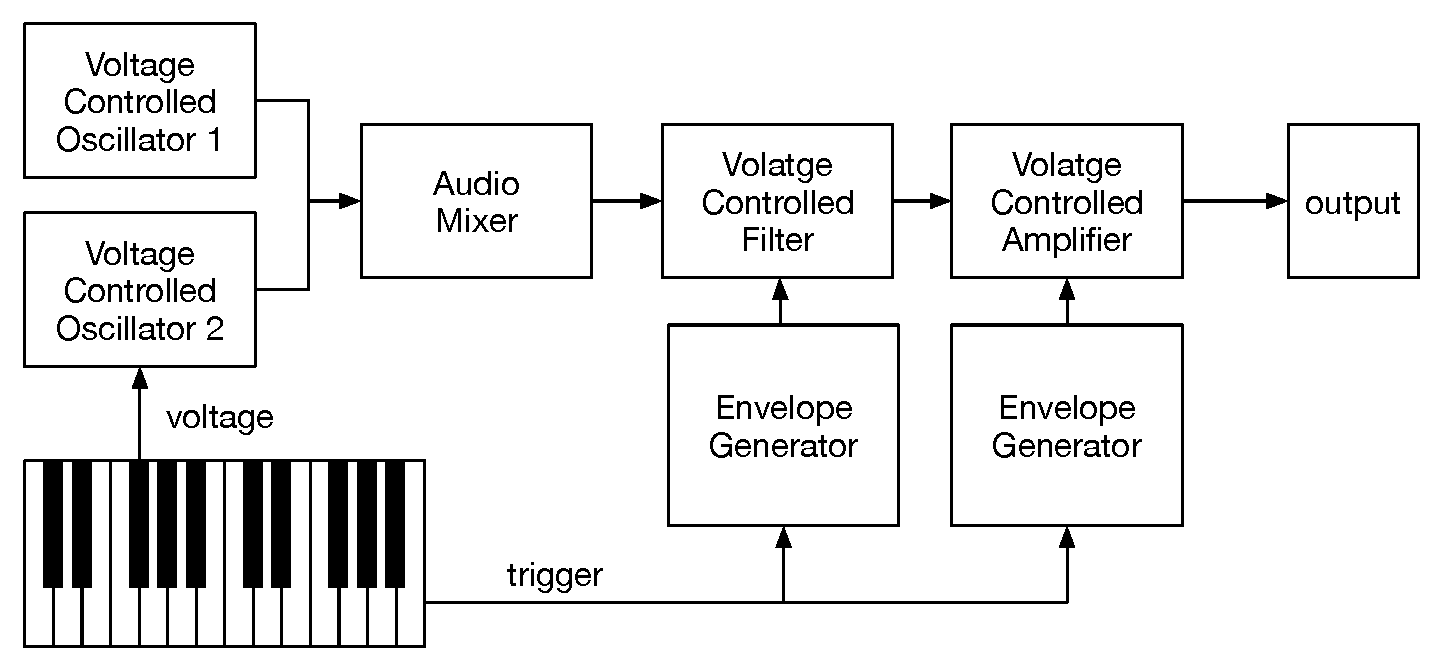
\includegraphics[width=\textwidth]{assets/synth_voice_block.pdf}
    \caption{Blockschaltbild einer subtraktiven Synthesizer-Stimme}
    \label{fig:synth_voice_block}
\end{figure}

Die spannungsgesteuerte Oszillatoren (voltage controlled oscillators, VCO) erzeugen einfache Wellenformen in der Tonhöhe, die auf der Tastatur gespielt wird. Der Benutzer kann in der Regel zwischen einer Kombination aus Sägezahn-, Rechteck- oder Dreieck-Wellenform wählen. Die Frequenzen oder die Klangfarbe der Wellenformen können dann durch die folgenden Filter und Amplituden-Blöcke moduliert werden.

Der erste Eindruck könnte sein, dass die Modellierung des Oszillators einfach ist. Eine digital erzeugte Rechteck- oder Sägezahn-Wellenform sollte leicht zu implementieren sein. Die 5-kHz-Sägezahn-Wellenform beispielsweise würde sich alle 8,82 Samples wiederholen bei einer Taktrate von 44,1 kHz. So würde die Wellenform sich linear von -1,0 auf 1,0 erhöhen, dann zurückspringen auf -1.0 und wieder von vorn beginnen.  Was bedeutet aber 0,82 Samples in einem diskreten digitalen System? A veranschaulicht das Problem. Die linke Spalte zeigt einen Abschnitt einer idealisierten 5kHz-Sägezahnwellenform und den entsprechenden Frequenzinhalt. Oberhalb der Grundfrequenz 5 kHz sind Oberwellen, die weit über 100 kHz hörbar sein werden. Die rechte Spalte zeigt den gleichen Abschnitt einer 5kHz-Sägezahnwellenform in einer mit 44,1kHz getakteten diskreten Umgebung. Die Wellenform selbst ist verzerrt und die höheren Harmonien sichtbar von der 22,05 kHz Nyquist-Grenze nach unten reflektiert.


\begin{figure}[H]
    \centering
    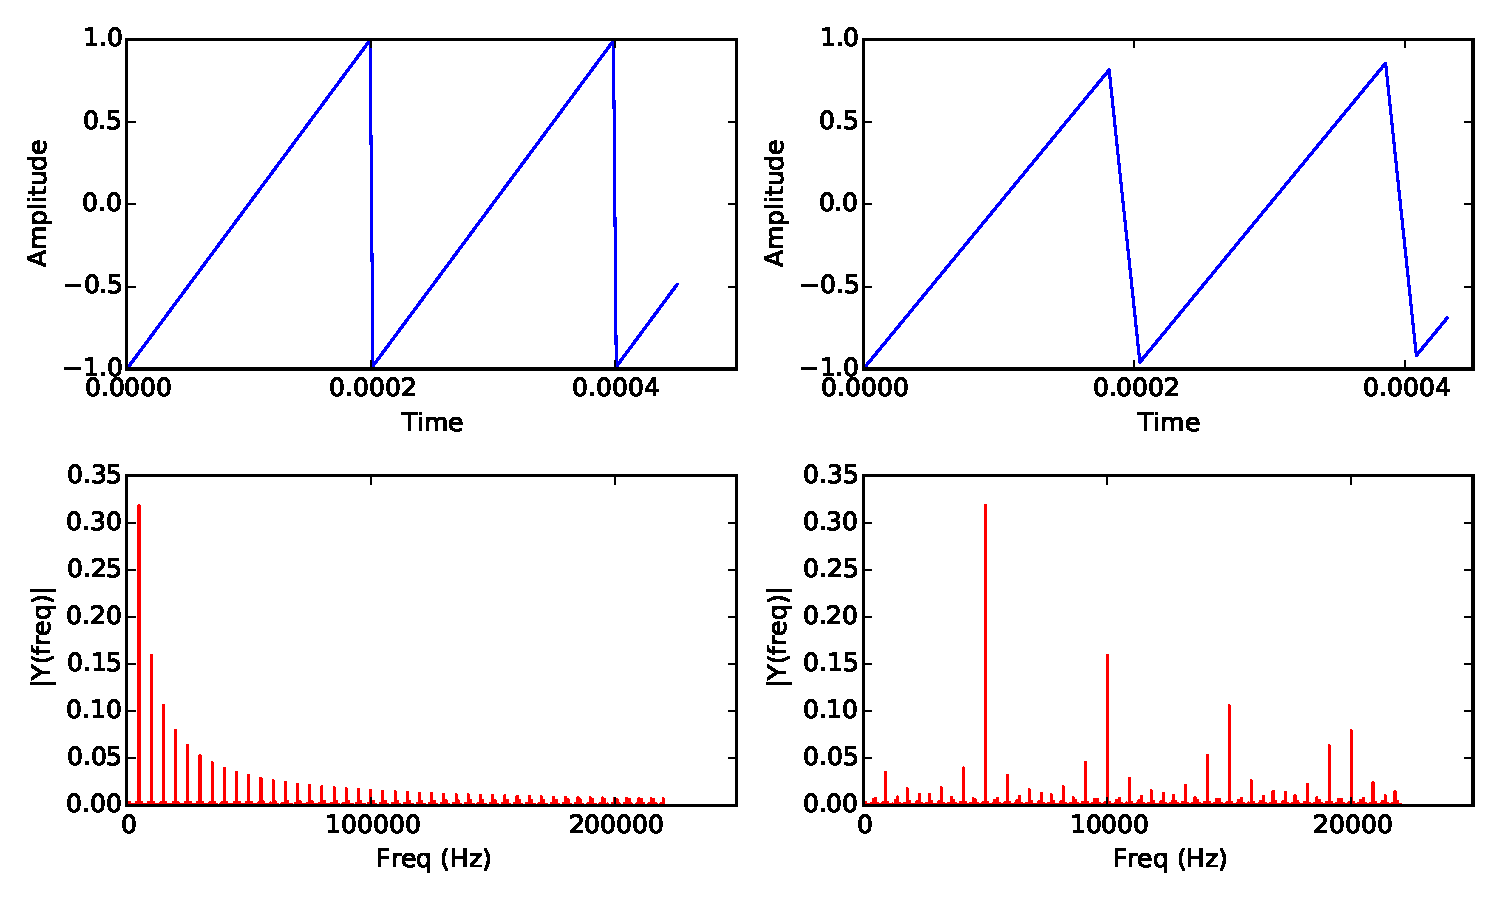
\includegraphics[width=\textwidth]{plots/graphics/sawtooth.pdf}
    \caption{Ideale und Aliased 5kHz-Sägezahnwellenform}
    \label{fig:aliasing_sawtooth}
\end{figure}

Es gibt verschiedene Verfahren zur Beseitigung oder Verminderung von Aliasing. Die effektivste ist es, die Oberwellen mit einer Reihe von Sinus-Wellen bis zu der Nyquist-Grenze oder die Hälfte der Abtastrate des Systems zu konstruieren, aber dies ist sehr rechenintensiv. Weniger CPU-intensive Strategien sind Oversampling,  Bandbegrenzung oder andere Aliasing-Unterdrückungsmethoden.





